\documentclass[xcolor={svgnames}]{beamer}

\setlength{\unitlength}{1cm} 
\usetheme{Boadilla}

    \usepackage[english]{babel}
    \usepackage[utf8]{inputenc} 
    \usepackage{csquotes}
    \usepackage{amsmath, amssymb}
    \usepackage{graphicx}
    \usepackage{tikz} 
    

    \setlength{\parindent}{0em}
    \setlength{\parskip}{0.5em}

    % Graphs
    \usetikzlibrary{positioning}
    \tikzset{main node/.style={circle, draw,minimum size=1cm,inner sep=3pt},}

    % Math commands
    \newcommand{\E}{\mathbb{E}}
    \newcommand{\norm}[1]{\left\lVert#1\right\rVert}
    \newcommand{\R}{\mathbb{R}}

    % Bibliography
    \usepackage[bibencoding=utf8, style=apa]{biblatex}

    \bibliography{../../../Desktop/bibliographies/thesis}


\title[Trophic analysis of Electricity markets]{Trophic Analysis of a\\ Prosumer Electricity Market}
\subtitle{Research proposal}
\author{Andrea Titton}
\institute{Tinbergen Institute}
\date{\today}

\begin{document}

\frame{\titlepage}

\begin{frame}{Advent of prosumers}
    Green energy transition,
    \begin{itemize}\setlength\itemsep{1em}
        \item Electricity \textbf{production} becomes prerogative of households
        \item Issues and benefits with centralized grid firms (e.g. ERCOT in Texas)
        \item Weather shocks and uncertainty among risk averse consumers
    \end{itemize}
\end{frame}

\begin{frame}{Research question}
    Under which conditions is a network of prosumer markets \textbf{stable}?

\end{frame}

\begin{frame}{Modelling idea}
    The model should capture
    \begin{itemize}\setlength\itemsep{1em}
        \item Tension between risk aversion of electricity demand, uncertainty of endowments, and grid firms bottleneck
        \item Given the network structure, which pricing mechanism can ``ease the pain'' ?
        \item Does bounded rationality (laziness of prosumers) poses a threat to stability?
    \end{itemize}
\end{frame}


\begin{frame}{Example electricity markets (\citeauthor{Parag2016})}
\begin{minipage}{.45\linewidth}
    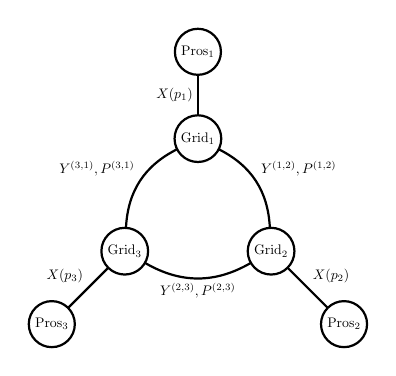
\begin{tikzpicture}[-, thick, scale=0.6, every node/.style={scale=0.5}]
        % Grids
        \node[main node] (1) {Grid$_1$};
        \node[main node] [below right = 1cm and 0.5cm of 1] (2) {Grid$_2$};
        \node[main node] [below left = 1cm and 0.5cm of 1] (3) {Grid$_3$};
        % Local markets 
        \node[main node] [above = 0.5 of 1] (5) {Pros$_1$};
        \node[main node] [below right = 0.5 and 0.5 of 2] (6) {Pros$_2$};
        \node[main node] [below left = 0.5 and 0.5 of 3] (7) {Pros$_3$};
        % Paths
        \path[draw,thick]
        (1) edge [bend left] node [above right] {$Y^{(1, 2)}, P^{(1, 2)}$} (2)
        (2) edge [bend left] node [below] {$Y^{(2, 3)}, P^{(2, 3)}$} (3)
        (3) edge [bend left] node [above left] {$Y^{(3, 1)}, P^{(3, 1)}$} (1)
        (1) edge node [left] {$X(p_{1})$} (5)
        (2) edge node [above right] {$X(p_{2})$} (6)
        (3) edge node [above left] {$X(p_{3})$} (7);
    \end{tikzpicture}
\end{minipage}
\begingroup \fontsize{10pt}{12pt}\selectfont
\begin{minipage}{.5\linewidth}
    \begin{itemize} \setlength\itemsep{1em}
        \item Local \textbf{prosumers} market \begin{itemize}
                  \item Endowed electricity
                  \item Can trade with local \textbf{grid firm}
                  \item Heterogenous in need and price forecasting rule \nocite{Hommes2013}
                  \item Risk averse
                  \item Cash in hand constraint
              \end{itemize}
        \item \textbf{Grid firms} \begin{itemize}
                  \item Can trade within network
                  \item Profit maximizing
                  \item Rational
              \end{itemize}
    \end{itemize}
\end{minipage}
\endgroup
\end{frame}

\begin{frame}{Prosumers}
    Prosumer optimization problem, suppressing notation $i$,
    \begin{equation*}
        \begin{split}
            V(e_t) &= \sup_{x_t \in \R} \left\{\underbrace{u(x_t + e_t)}_{\text{electricity consumption}} + \beta \cdot \E_t V( e_{t+1} ) \right\} \\
            \\
            \textit{s.t. } &m_{t+1} = m_{t} - \overbrace{p_{t}}^{\text{price on grid}} \cdot \underbrace{x_{t}}_{\text{electricity demand}}, \ \underbrace{m_t  \geq 0}_{\text{cash in hand}}
        \end{split}
    \end{equation*}
\end{frame}

\iffalse
    \begin{frame}{Prosumers' type}

        Prosumers can be either can be either fundamentalists or chartists, $h \in \{f, c\}$. This determines their price expectation,

        \begin{equation}
            \begin{split}
                \E_t[p_{t+1}] &= \psi_h \cdot p_t \\
                &0 < \psi_f < 1 \text{ and } \psi_c > 1
            \end{split}
        \end{equation}


        The decision to switch between types is driven by how well that type performed.

        At each time step there is a fraction of fundamentalists and chartists in local market, such that $N_c + N_f = N$.

    \end{frame}
\fi

\begin{frame}{Partial equilibrium in local market}

    Via Euler equation, one can find policy function,

    \begin{equation}
        m_{t+1} = g(m_t, p_t \vert e_t) \implies x_{t+1} = \frac{m_t - g(m_t, p_t \vert e_t)}{p_{t+1}}
    \end{equation}

    Aggregating over the two types yields the total demand (or supply) of electricity of the grid

    \begin{equation}
        X_{t+1}(p_{t+1}, p_t \vert e_t) = \sum_{i \in c} x_{i, t+1} + \sum_{j \in f} x_{j, t+1}
    \end{equation}

\end{frame}


\begin{frame}{Equilibrium prosumer energy demand}
    \begin{figure}
        \centering
        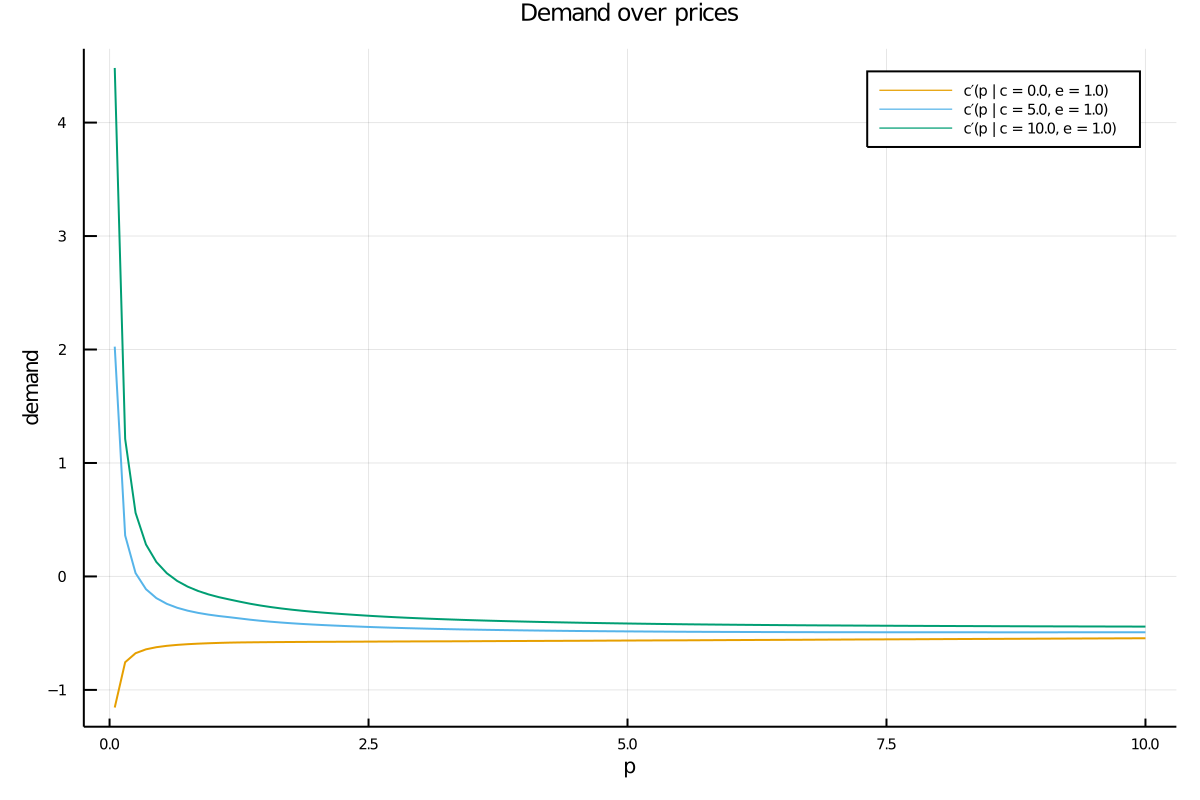
\includegraphics[width=0.9\textwidth]{../../plots/markets/pricedemand.png}
    \end{figure}
\end{frame}

\begin{frame}{Simulated local market demand}

    \begin{figure}
        \centering
        \begin{minipage}{.5\textwidth}
            \centering
            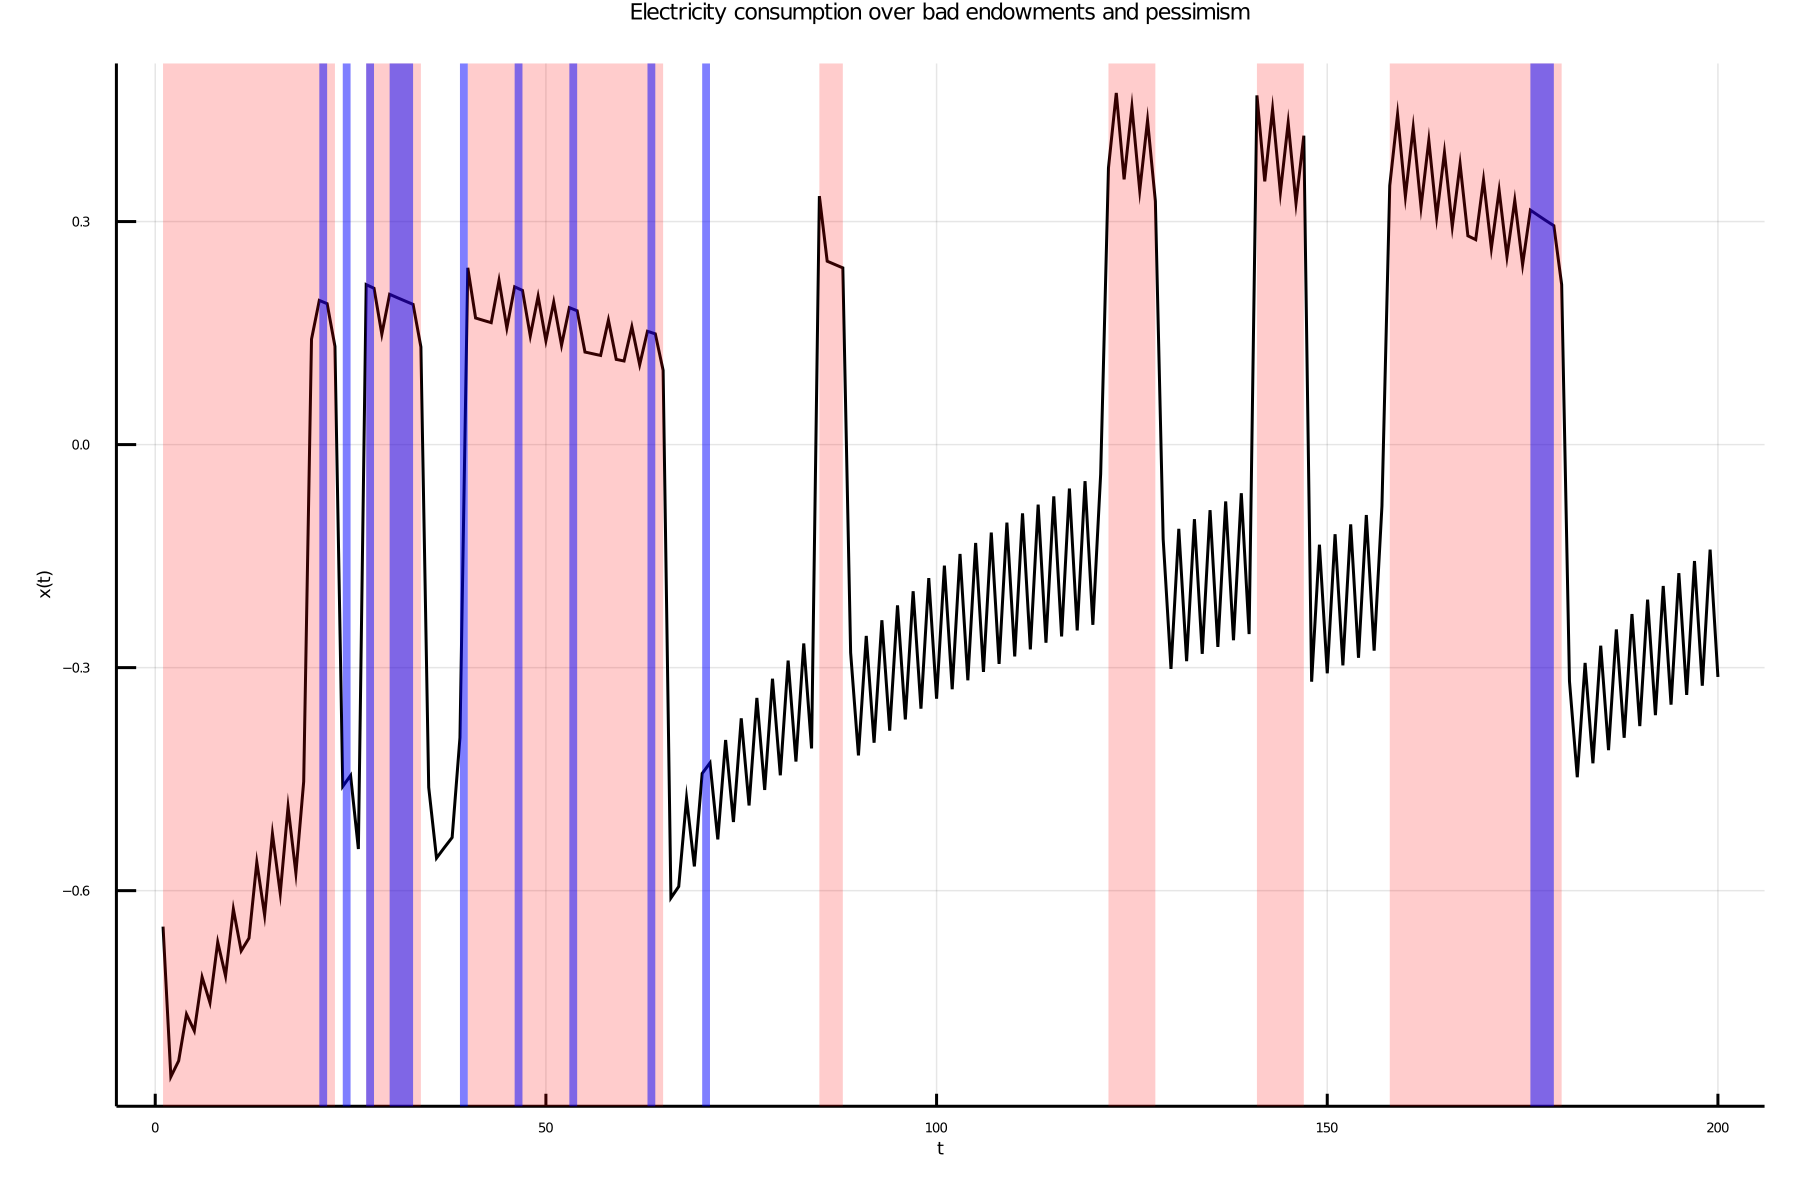
\includegraphics[width=\linewidth]{../../plots/markets/simul.png}
        \end{minipage}%
        \begin{minipage}{.5\textwidth}
            \centering
            \includegraphics[width=\linewidth]{../../plots/markets/kde.png}
        \end{minipage}
    \end{figure}

\end{frame}

\begin{frame}{Grid firms}
    Let $N(i)$ be the neighbors of grid firm $i$. Then the firm's profit are,
    \begin{equation}
        \Pi(p_t) = X_{t}(p_t) \cdot p_t - \sum_{j \in N(i)} Y^{(i, j)}_{t} \cdot \underbrace{P^{(i, j)}_t}_{\text{prices on network}},
    \end{equation}
    subject to,
    \begin{equation}
        \underbrace{X_t}_{\text{local demand}} =  \underbrace{\sum_{j \in N(i)} Y^{(i, j)}_{t}}_{\text{energy bought from firm $j$}}
    \end{equation}
\end{frame}

\begin{frame}{Equilibrium}
    \begin{minipage}{.35\linewidth}
        \begin{itemize}
            \item Optimizing prosumers and firms
            \item Feasibility requires $\sum_{i \in \mathcal{G}} X^i_t = 0$
        \end{itemize}
    \end{minipage}
    $\implies$
    \begin{minipage}{.55\linewidth}
        \begin{itemize}
            \item Discrete time dynamical system: \begin{equation*}(X^1, \ldots X^n)_{t+1} = f((X^1, \ldots X^n)_t)\end{equation*}
            \item Non-analytical but computable $f$
        \end{itemize}
    \end{minipage}
    \vfill
    \centering
    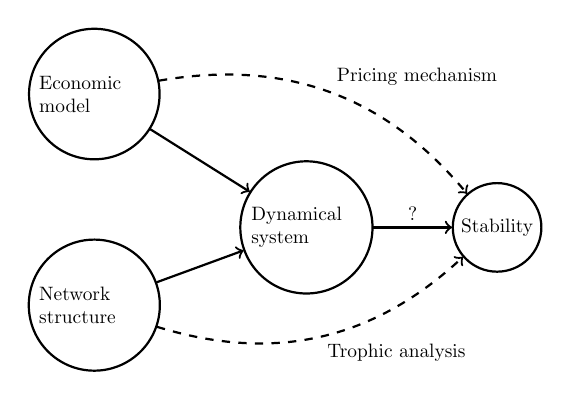
\begin{tikzpicture}[->, thick, every node/.style={scale=0.7}]
        % Nodes
        \node[main node] (1) [text width=2cm]  {Economic model};
        \node[main node] [below = 1cm of 1, text width=2cm] (2) {Network structure};
        \node[main node] [below right = 0.5cm and 1.5cm of 1, text width=2cm] (3) {Dynamical system};
        \node[main node] [right = 1cm of 3] (4) {Stability};
        % Paths
        \path[draw,thick]
        (1) edge node {} (3)
        (2) edge node {} (3)
        (3) edge node [above] {?} (4)
        (1) edge [dashed, bend left] node [above right] {Pricing mechanism} (4)
        (2) edge [dashed, bend right] node [below right] {Trophic analysis} (4);
    \end{tikzpicture}

\end{frame}

\begingroup
% TODO section
\setbeamercolor{background canvas}{bg=AliceBlue}
\begin{frame}{\textit{Steps forward}: Trophic analysis}
    Building on \citeauthor[]{MacKay2020}. Measure of hierarchical structure among nodes.

    \begin{columns}
        \begin{column}{.49\textwidth}
            \begin{figure}
                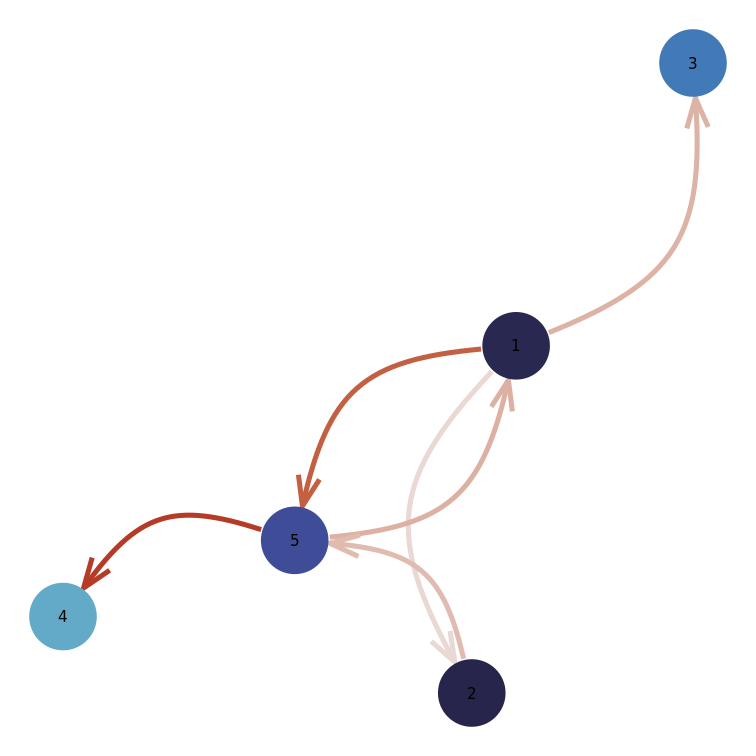
\includegraphics[width=0.8\linewidth,height=0.8\textheight,keepaspectratio]{../../plots/presentations/lv-network.png}
            \end{figure}
        \end{column}
        \begin{column}{.48\textwidth}
            The trophic level $h$ solves,
            \begin{equation*}
                \begin{split}
                    \Lambda h &= \overbrace{v}^{\textit{imbalance}} \text{ where }\\
                    \Lambda &:= \underbrace{diag(u)}_{\textit{total weight}} - W - W^T
                \end{split}
            \end{equation*}
            \begin{itemize}
                \item Ecologic stability
                \item Neural cascade
                \item Epidemics
                \item Linked to properties of dynamical systems
            \end{itemize}
        \end{column}
    \end{columns}
\end{frame}

\begin{frame}{\textit{Steps forward}: Strategic bargaining on network}
    \begin{itemize} \setlength\itemsep{1em}
        \item \citeauthor{Lopes2011} find evidence for bilateral bargaining among grid firms over prices, $(P_{1, 2}, P_{1, 3}, \ldots, P_{n-1, n})$
        \item Which price mechanism arises (Cooperative bargaining theory)? Is it efficient and/or stable?
        \item Common pricing solutions: \begin{itemize}\setlength\itemsep{0.5em}
                  \item \textit{Day-ahead}
                  \item \textit{Intra-day}
                  \item \textit{Feed-in}
                  \item \textit{P2P}
              \end{itemize}
    \end{itemize}
\end{frame}

\begin{frame}{\textit{Steps forward}: Model calibration}
    \begin{itemize}\setlength\itemsep{1em}
        \item Indirect inference of prosumer's parameters. Aggregate energy demand on micro-grids from \citeauthor{Fridgen2018}.
        \item Method of moment of grid firm's parameters with grid prices. \textit{Issue:} Surely misspecified firm's budget constraint
        \item Model validation on residual moments (household's energy production)
    \end{itemize}
\end{frame}

\endgroup


\begin{frame}[allowframebreaks]{Bibliography}
    \printbibliography
\end{frame}

\end{document}